\section{Cabo de Guerra}

%%%%%%%%%%%%%%%%%%%%%%%%%%%%%%%%%%%%%%%%%%%%%%%%%%%%%%%%%%%%%
\subsection{Descrição}

\textcolor{red}{Melhorar o enunciado ... mas o outros estão melhores}\\

Várias crianças se encontram para 
 brincadeira do cabo-de-guerra no pátio da escola. Como será
 feita a divisão entre as  duas equipes?   ``{\em Por peso}''\/ grita o mais eufórico. Que seja feita a divisão dos times  sobre uma sequência/lista de peso tal como:
 
\begin{center}
\begin{tabular}{|c|c|c|c|c|}
\hline
$Joao_1$ & $Pedro_2$ & $Manoel_3$ & .... & $Zeca_n$ \\ \hline
45 & 39 & 79 & .... & 42  \\ \hline
\end{tabular}
\end{center}

\ding{224} Preencha a tabela acima com inteiros e valores de sua família.

\ding{224}  Sim, por peso, todos concordaram,
 ``{\em exceto que a divisão deveria respeitar o critério $|N_A - N_B| \le 1$}'', disse o 
mais cauteloso. Sim, nenhum time poderia duas crianças a mais que ou outro time. 

%%%%%%%%%%%%%%%%%%%%%%%%%%%%%%%%%%%%%%%%%%%%%%%%%%%
\subsection{Especificação}

Que seja feita a divisão:

 
\begin{center}
\begin{tabular}{|c|c|c|c|c|}
\hline
$Joao_1$ & $Pedro_2$ & $Manoel_3$ & .... & $Zeca_n$ \\ \hline
45 & 39 & 79 & .... & 42  \\ \hline
\end{tabular}
\end{center}

\begin{itemize}
\item Divisão  por peso
\item Respeitar  critérios como: $|N_A - N_B| \le 1$
\item Todos devem brincar

\item \textsf{Bem, esta simples {\bf \underline{restrição}} ({\bf $|N_A - N_B| \le 1$}), de nosso cotidiano tornou um simples problema em mais uma questão combinatória.
 Um arranjo da ordem de  $\frac{n!}{(n/2)!}$.
 Casualmente, nada trivial  para grandes valores! }
 \end{itemize}


\ding{224} Dois detalhes:

\begin{enumerate}
\item Na tabela de pesos, use valores {\bf inteiros};

\item Use os pesos de seus familiares para completar esta tabela
com um quantidade significativa;

\item No lugar de {\em array} como estrutura base, use {\em sets} para armazenar
e manipular estes valores. Com certeza ficará mais  {\em elegante}, e 
possivelmente mais ineficiente. Teste e comprove!

\end{enumerate}

%%%%%%%%%%%%%%%%%%%%%%%%%%%%%%%%%%%%%%%%%%%%%%%%

\subsection{Modelagem}

 \begin{itemize}

  \item Usando uma variável de decisão: análogo a árvore do SAT  
 
\begin{center}
\begin{tabular}{|l|c|c|c|c|c|}
\hline
Nomes ($n_i$): & $n_1$ & $n_2$ & $n_3$ & .... & $n_n$ \\ \hline
Peso ($p_i$): & 45 & 39 & 79 & .... & 42  \\ \hline
Binária ($x_i$): & 0/1 & 0/1 & 0/1 & .... & 0/1  \\ \hline
\end{tabular}
\end{center}
  
\item Assim $N_A \approx N/2$, $N_B \approx N/2$  e  $|N_A - N_B| \le 1$   

\item $x_i = 0$: $n_i$ fica para o time $A$
\item $x_i = 1$: $n_i$ fica para o time $B$
\item Logo a soma:
$$\sum_{i=1}^n x_i p_i$$ é o peso total do time $B$ ($P_B$)
  
  \end{itemize}

%%%%%%%%%%%%%%%%%%%%%%%%%%%%%%%%%%%%%%%%%%%%%%%%%

  \begin{itemize}
  \item Falta encontrar peso total do time $A$ ($P_A$), dado por: 

  \item $P_A = P_{total} - P_B$
  
  \item  ou $$P_A = \sum_{i=1}^n p_i - \sum_{i=1}^n x_i p_i$$   

  \item Finalmente, aplicar uma minimização  na diferença: $|P_A - P_B|$
  
%%  \item A seguir, tudo isto em código:
  
  \end{itemize}

%%%%%%%%%%%%%%%%%%%%%%%%%%%%%%%%%%%%%%%%%%%%%%%%%
\subsection{Estratégia}%%% de Implementação}

Uma árvore de decisão binária ............ descreva como
voce implementou ou a fundamentacao

\begin{figure}[ht!]
 \centering
 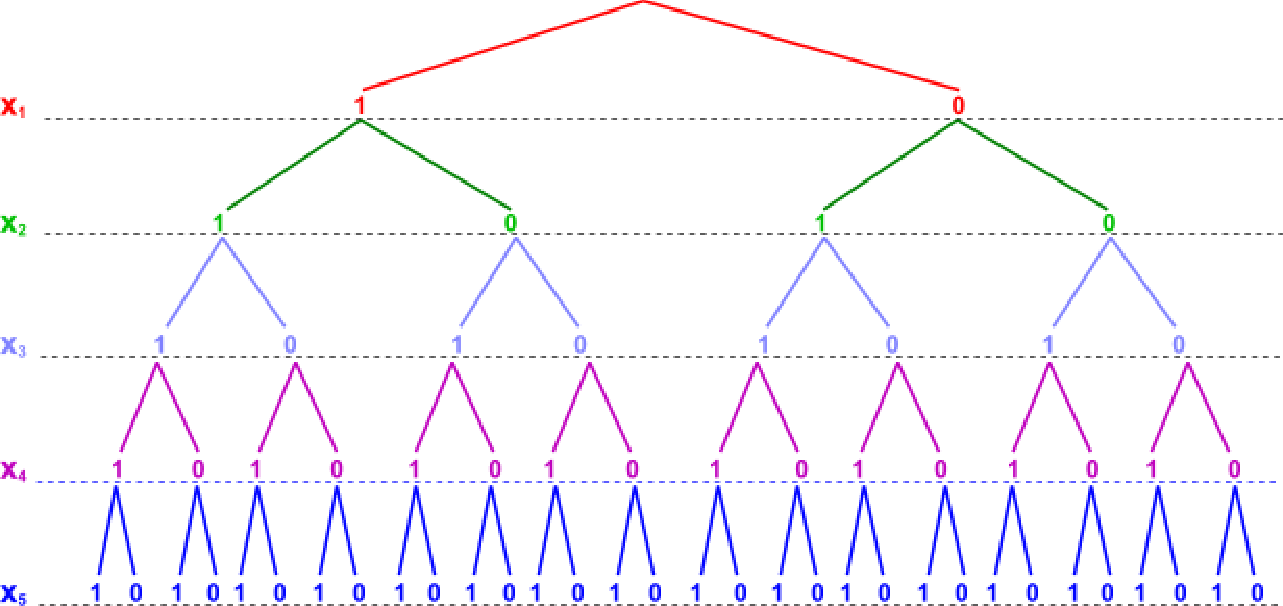
\includegraphics[width=0.7\textwidth , height=0.3\textheight]{binary_tree04.pdf}
\caption{Se $x_i=0$, então $n_i$ segue para o time $A$, caso  $x_i=1$, então  $n_i$ vai para o time $B$} 
%\label{}
\end{figure}

%%%%%%%%%%%%%%%%%%%%%%%%%%%%%%%%%%%%%%%%%%%%%%%%%
\subsection{Implementação}

O código fonte se encontra em:

\url{https://github.com/claudiosa/CCS/tree/master/minizinc/cabo_de_guerra.mzn}

%%%%%%%%%%%%%%%%%%%%%%%%%%%%%%%%%%%%%%%%%%%%%%%%%
\subsection{Resultados e Análise}


Considerando pesos aleatórios de 1 a 150 para as pessoas

Usando um \textit{solver} médio do Minizinc (\textit{G12 lazyfd}) padrão:

\begin{table}
  \caption{Resultados ...................}
   \label{tab:}
  
  \begin{center}
  \begin{tabular}{ l | c |c | r }
    \hline  \hline 
    $n$ & tempo & $P_A$ & $P_B$\\ \hline     \hline 
     5 & 40msec & 276 & 278 \\ \hline
    10 & 46msec & 518 & 519 \\ \hline
    25 & 98msec & 1198 & 1197 \\ \hline
    50 & 411msec & 2290 & 2291 \\ \hline
    75 & \textbf{\textcolor{red}{2s 485msec}} & 3133 & 3133 \\ \hline
    100 & 470msec & 4142 & 4142 \\ \hline 
    125 & \textbf{\textcolor{red}{7s 2msec}} & 4992 & 4992 \\ \hline 
    150 & 605msec & 5823 & 5823 \\ \hline 
    175 & 642msec &   6777 &  6778 \\ \hline 
    200 & $>$ 10min & -- & -- \\ \hline \hline
  \end{tabular}
  
\end{center}

\end{table}
Referência: cpu 4-core, 4 G ram, SO: Linux-Debian

%%%%%%%%%%%%%%%%%%%%%%%%%%%%%%%%%%%%%%%%%%%%%%%%%%%%%%%%%%%%%%%%%%%%%%%%%%%%%%%%%%%%%%%%%%%%%%%%%%%%%%%%%%%%%%
